\documentclass[a4paper,10pt]{report}
\usepackage[T1]{fontenc}
\usepackage[utf8]{inputenc}
\usepackage[francais]{babel}
\usepackage{url}
\usepackage{graphicx}
\usepackage{hyperref}
\usepackage{fancyhdr}

\fancyhf{}

\title{Tutorat Git}

\lhead{C2R1}
\chead{Tutorat Git}
\rhead{page \thepage}

\begin{document}
\renewcommand{\chaptername}{Partie}

\begin{titlepage}
\vspace{-3cm}\hspace{-2cm}
\includegraphics[scale=0.4]{C2R1}
\begin{center}
\vspace{2cm}
{\fontfamily{phv}\selectfont
\Large{C2R1}\\
\vspace{0.5cm}
\Huge{Tutorat Git}}\\
\end{center}
\begin{flushright}
 \vfill
{\fontfamily{phv}\selectfont
\large{Version du \today}}
\end{flushright}
\end{titlepage}

\pagestyle{fancy}

\tableofcontents
\newpage

\chapter{Introduction}
  \section{Histoire}
    \subsection{Versionnage de code?}
Lorsqu'on travaille \`a plusieurs sur un projet, il est fr\'equent de devoir travailler au m\^eme moment. C'est ce \`a quoi servent les gestionnaires de version. Ils permettent \`a chaque d\'eveloppeur de travailler localement, puis de l'envoyer aux autres d\'eveloppeurs une fois leurs modifications finie.
    \subsection{Outils de versionnage}
Il existe de nombreux outils de versionnage de code. Les 3 plus connus sont sans doute Git, Mercurial et SVN.
      \subsubsection{SVN (subversion)}
Ce fut le plus utilisé pendant longtemps. Développé par la fondation Apache, il s'agit d'une amélioration d'un programme nommé CVS (très peu utilisé aujourd'hui). Le plus gros problème de SVN est qu'il s'agit d'un système centralisé. Un serveur contient donc le code, des clients travaillent dessus. Il n'y a qu'un seul versionning. C'est le gestionnaire de version utilis\'e notamment par Apache, freeBSD et sourceforge.
      \subsubsection{Mercurial}
Contrairement à SVN, il s'agit d'un système décentralisé. Chacun possède son propre \emph{repository} et publie son code sur le \emph{repository} public. Une autre différence avec SVN est qu'il utilise la notion de changeset. C'est à dire qu'il préfère garder en mémoire les changements appliqués que les versions des fichiers. Il est utilis\'e notamment par Mozilla (Firefox, Thunderbird, ...), Facebook, et adblock plus.
      \subsubsection{Git}
Git possède très peu de différences avec Mercurial, mais l'histoire a fait qu'il c'est plus imposé.
C'est en partie grâce à Linus Torvalds qui en a fait la pub et des projets comme github que nous allons utiliser dans le reste du tutorat.
C'est le gestionnaire de version utilis\'e par l'\'equipe de d\'eveloppeurs du noyeau linux.\\

Pour plus d'informations sur les différences entre mercurial et Git, vous pouvez vous référer à ces articles~: \url{http://importantshock.wordpress.com/2008/08/07/git-vs-mercurial/}, \url{http://www.rockstarprogrammer.org/post/2008/apr/06/differences-between-mercurial-and-git/}.
  \section{Installation du client git}
    \subsection{Windows}
Lancez le programme que vous pouvez trouver sur cette page : \url{http://msysgit.github.io} ou \url{http://www.git-scm.com/}
    \subsection{Linux}
\verb|apt-get install git| ou \verb|yum install git| selon la distribution
    \subsection{Mac OS}
\verb|sudo port install git-core +svn +doc +bash_completion +gitweb|
  \section{Choix du serveur git}
Pour la suite de ce tutorat, il vous faut créer un compte github : \url{https://github.com/}.
Vous pouvez aussi vous intéresser à gitlab : \url{https://about.gitlab.com/}

\chapter{Manipulation basique de git}
  \section{D\'ebut du projet}
    \subsection{Cr\'eer le d\'ep\^ot}
Pour cr\'eer le d\'ep\^ot, il faut initialiser un dossier. Ceci se fait avec la commande \verb|git init| (cette \'etape est optionnelle avec github). Ensuite, il faut cr\'eer le d\'ep\^ot sur le serveur.\\
Sur Github, ceci se fait avec un formulaire, accessible en cliquant sur le bouton \emph{create repository}, \`a c\^ot\'e de la liste des d\'ep\^ots d\'ej\`a existants.\\
\begin{figure}[h!]
  \begin{center}
    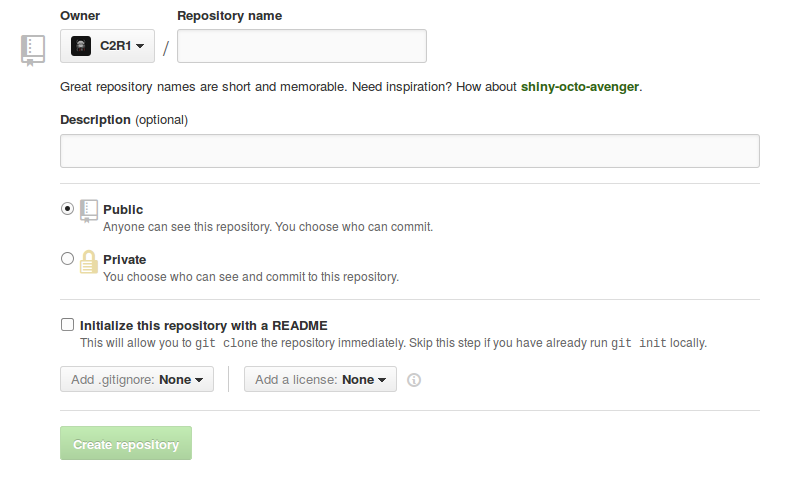
\includegraphics[scale=0.3]{images/createRepoForm}
    \caption{Formulaire de cr\'eation de d\'ep\^ot}
    \label{creationRepo}
  \end{center}
\end{figure}

Nous avons alors un formulaire de cr\'eation de d\'ep\^ot (cf figure \ref{creationRepo}), qui nous demande~:
\begin{itemize}
 \item le nom du d\'ep\^ot (\emph{Repository name})
 \item une description (optionnelle)
 \item s'il faut initialiser le d\'ep\^ot (\`a ne pas cocher si vous avez fait \verb|git init|).
\end{itemize}

    \subsection{R\'ecup\'erer un d\'ep\^ot existant}
Pour r\'ecup\'erer un d\'ep\^ot existant, il faut connaitre l'\emph{url} du d\'ep\^ot. Par exemple \url{https://github.com/C2R1/Tutorats.git}. Vous trouverez cette addresse sur la page du d\'ep\^ot sur github, sous le nom \emph{HTTPS clone URL}.\\

il faut alors aller dans le dossier o\`u l'on veut cloner le d\'ep\^ot, et effectuer la commande \verb|git clone <URL>|.\\
Ainsi, pour notre exemple~: \verb|git clone https://github.com/C2R1/Tutorats.git|.

    \subsection{README}
Le README est un fichier de présentation du projet. Généralement, on y décrit son installation, les fonctionnalités à venir, comment contribuer, la licence, ...
  \section{Premier commit}
Une fois que l'on a le d\'ep\^ot clon\'e sur son ordinateur, on peut commencer \`a coder. Cependant, les modifications ne se font pas en temps r\'eel sur le serveur. Ainsi, il faut connaitre quelques commandes pour r\'ecup\'erer les modifications faites par les autres d\'eveloppeurs, et pouvoir leur envoyer nos modifications.
     \subsection{R\'ecup\'erer les modifications depuis le serveur}
Pour r\'ecup\'erer les modifications, il faut utiliser la commande \verb|git pull|.
     \subsection{Envoyer les modifications vers le serveur}
Pour envoyer les modifications au serveur, il faut tout d'abord dire \`a git les fichiers qui ont \'et\'es ajout\'es depuis la derni\`ere modification. Ceci se fait avec la commande \verb|git add <fichiers>|. Par exemple, pour ajouter tous les nouveaux fichiers, on peut utiliser \verb|git add *|.\\

Ensuite, il faut ``enregistrer'' les modifications localement. On dit alors qu'on \emph{commit} les changements. La commande est donc \verb|git commit <fichiers>|, en sp\'ecifiant les fichier \`a \emph{commit}. Pour enregistrer les modifications de tous les fichiers, on utilise l'option \verb|-a| (pour \emph{all}), et ainsi~: \verb|git commit -a|.\\
Durant un commit, il faut expliquer les changements effectu\'es. C'est l'utilit\'e du \emph{commit message}. On peut sp\'ecifier ce message en utilisant l'option \verb|-m <message>|. soit~: \verb|git commit -m <message>|.\\
Si l'on ne sp\'ecifie pas de message avec l'option \verb|-m|, \verb|git| lancera un \'editeur de texte (\verb|vi| par d\'efaut) pour \'ecrire le message. En cas de message vide, le commit ne peut se faire.\\

Enfin, il faut envoyer ses modifications au serveur. C'est l'utilit\'e de la commande \verb|git push|. \\

Par exemple, pour ``dire'' au serveur qu'on a ajout\'e le fichier \verb|c2r1.dtc|, on utilisera la suite de commande~:
\begin{verbatim}
>> git add c2r1.dtc
>> git commit -am "ajout du fichier c2r1.dtc"
>> git push
\end{verbatim}

Soit~:
\begin{itemize}
 \item On ``avertit'' git qu'on ajoute le fichier,
 \item On \emph{commit} les changements de tous les fichiers (\verb|a|), avec un message (\verb|m|),
 \item On envoie les modifications au serveur.
\end{itemize}


     \subsection{diff/ignore}
Pour obtenir tous les changements effectués depuis le dernier commit. Voici la forme d'un fichier diff :
\begin{verbatim}
     diff --git a/apps/system/js/sound_manager.js b/apps/system/js/sound_manager.js
index b796d13..3847b93 100644
--- a/apps/system/js/sound_manager.js
+++ b/apps/system/js/sound_manager.js
@@ -686,7 +686,11 @@
     };
   }
 
-  function setVibrationEnabled(enabled) {
+  function setVibrationEnabled(enabled) {    
+    //vibrate
+    if ('vibrate' in navigator && enabled) {
+      navigator.vibrate([200, 100, 200]);
+    }
     setVibrationEnabledCount++;
     SettingsListener.getSettingsLock().set({
       'vibration.enabled': enabled
\end{verbatim}   
Note : On peut aussi obtenir la différence entre 2 commits avec cette commande. \\
On y trouve donc le numéro du commit, les fichiers modifiés, les lignes supprimées ainsi que les lignes ajoutées.
  \section{Historique}
\chapter{Manipulation avancée}
	\section{Plus d'informations sur le fonctionnement de git}
	Quand vous commitez avec git, git enregistre un objet qui contient un pointeur vers vos changements, l'auteur, le message de commit et un lien vers zéro parent si c'est le commit initial, 1 parent pour un commit classique, plus pour un commit résultant d'un merge entre 2 ou plusieurs branches.
\begin{figure}[h!]
  \begin{center}
    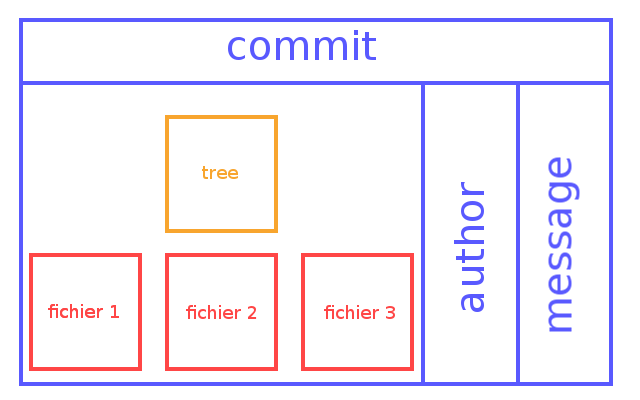
\includegraphics[scale=0.3]{images/objetcommit}
    \caption{Forme d'un objet commit}
    \label{obCommit}
  \end{center}
\end{figure}
	Un projet sera donc représenté par une suite de ces objets. Avec un pointeur nommé HEAD représentant l'endroit ou l'utilisateur se trouve.
\begin{figure}[h!]
  \begin{center}
    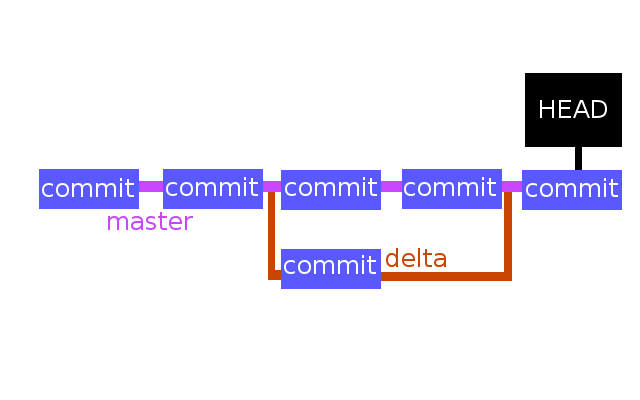
\includegraphics[scale=0.3]{images/git}
    \caption{Représentation d'un git}
    \label{obgit}
  \end{center}
\end{figure}

  \section{branch}
     \subsection{créer sa branche}
     Pour créer une branche (et plus généralement pour gérer des branches) il suffit d'utiliser la commande \verb|git branch|. Une autre méthode plus rapide et d'utiliser \verb|git checkout -b <nom de la branche>| qui va se charger de créer la branche et de se placer dessus. Pour se placer sur une branche qui existe, il faut utiliser \verb|git checkout <nom de la branche>| :
\begin{figure}[h!]
  \begin{center}
    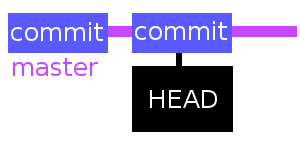
\includegraphics[scale=0.3]{images/prebranch}
    \caption{Avant git checkout -b}
    \label{obprebranch}
  \end{center}
\end{figure}
\begin{verbatim}
>> git checkout -b delta
\end{verbatim}
\begin{figure}[h!]
  \begin{center}
    
\includegraphics[scale=0.3]{images/afterbranch}
    \caption{Apr\`es git checkout -b}
    \label{obpostbranch}
  \end{center}
\end{figure}
     \subsection{fusionner}
     Pour fusionner deux branches, il faut utiliser \verb|git merge|.
     Exemple : On veut écraser une branche par une autre.\\
     1/ On se place dans le repository. Ici, il contient un dossier git et un fichier README.md
\begin{verbatim}
     >> ls
git  README.md
\end{verbatim}
     2/ On regarde l'historique pour chercher sur quel commit on veut se placer (ici initial commit)
\begin{verbatim}
>> git log
commit dcf387590eaf281c10ee7f989a690c223d0b125a
Author: AmarOk1412 <amarok@enconn.fr>
Date:   Tue Sep 30 13:11:15 2014 +0200

    git log

commit 2986c83edc7ca9f1bcbc565fbe13a14091005b1f
Author: n0m1s <n0m1s@homnomnom.fr>
Date:   Tue Sep 30 13:04:14 2014 +0200

    creation du depot

...

commit f1b4c0ebf59da0af7d782303f52bdae86c3d257b
Author: AmarOk1412 <amarok@enconn.fr>
Date:   Mon Sep 29 22:45:53 2014 +0200

    Initial commit
\end{verbatim}
    3/ On se place sur le commit. Et on créer une branche (ici on la nomme delta).
 \begin{verbatim}
>> git checkout f1b4c0ebf59da0af7d782303f52bdae86c3d257b
>> git checkout -b delta
Basculement sur la nouvelle branche 'delta'
>> git branch
* delta
  master
\end{verbatim}
    4/ On effectue quelques modifications et on les commit
\begin{verbatim}
>> echo someDiff > README.md 
>> git commit README.md -m "exemple"
[delta e1e999e] exemple
 1 file changed, 1 insertion(+), 2 deletions(-)
\end{verbatim}
    5/ Sur la branche qu'on souhaite garder on merge master avec une stratégie dite ours (ours
           This resolves any number of heads, but the resulting tree of the merge is always that of the current branch head, effectively ignoring
           all changes from all other branches. It is meant to be used to supersede old development history of side branches. Note that this is
           different from the -Xours option to the recursive merge strategy.
)
\begin{verbatim}
>> git merge -s ours master -m "ours attack"
Merge made by the 'ours' strategy.
\end{verbatim}
    6/ On se place sur la branche que l'on souhaite écraser (master ici). 
\begin{verbatim}
>> git checkout master
Basculement sur la branche 'master'
Votre branche est à jour avec 'origin/master'.
\end{verbatim}
    7/ Et on merge delta sur master
\begin{verbatim}
>> git merge --no-ff delta 
Message des modifications
\end{verbatim}
    8/ Et voilà, delta a écrasé master.
\begin{verbatim}
>> ls
README.md
\end{verbatim}


     \subsection{résoudre un conflit}
     \subsection{savoir qui a fait quoi}
     Pour savoir qui a fait quoi, il suffit de faire git log. On a alors accès à l'historique. un commit se présente de la forme : 
     "commit \no commit
Author: Auteur <mail>
Date:   Date

    message du commit"
  \section{Supprimer un commit}
  Pour supprimer un commit, il suffit de faire git revert \no du commit.
Exemple :
\begin{verbatim}
>>git log
"commit c610b4bbc6d631b798f158d2b999f0d0d0e108a4
Author: AmarOk1412 <amarok@enconn.fr>
Date:   Tue Sep 30 09:26:40 2014 +0200

    paragraph git diff + readme + Contribuer à un autre repo

commit 616b3c6843e6aaa42bcf3a6f680760d94dcee57d
Author: TheMrNomis <n0m1s@homnomnom.fr>
Date:   Tue Sep 30 09:23:07 2014 +0200

    titlepage

commit 781c38ff637c10166e6ef28d2574919cb865b7cf
Author: TheMrNomis <n0m1s@homnomnom.fr>
Date:   Tue Sep 30 08:41:26 2014 +0200

    plan du tutorat git

commit 1cd1ccccb53846f9763044da4bf50f26a5aebd10
Author: n0m1s <nomis@nosferapti.(none)>
Date:   Tue Sep 30 08:25:28 2014 +0200

    started git tutorial

commit f1b4c0ebf59da0af7d782303f52bdae86c3d257b
Author: AmarOk1412 <amarok@enconn.fr>
Date:   Mon Sep 29 22:45:53 2014 +0200

    Initial commit
"
\end{verbatim}
\verb|git revert f1b4c0ebf59da0af7d782303f52bdae86c3d257b| va donc nous supprimer le fichier README qui a été créé pendant ce commit.
  \section{Se positionner sur un commit}
  Pour se placer à un état précis, on utilise la commande git checkout comme pour se placer sur une branche. Il faut donc faire git checkout \no du commit (\verb|git checkout f1b4c0ebf59da0af7d782303f52bdae86c3d257b| par exemple) pour se placer sur un commit précis.
  IMAGE
  \section{Contribuer à un autre repository}
Généralement, il y a deux possibilités : 
* Contribuer sans coder, (graphisme, traduction, communication, ouverture de bugs)
* Coder
L'ouverture d'issues nécessite de regarder un minimum si l'issue n'a pas déjà été ouverte, de détailler son probleme et de bien regarder la version qu'on utilise.
Pour programmer, il faut forker le dépot et le récupérer en local.
Puis il suffit de créer sa branche, de réaliser les modifications nécessaires.
Quelques fois, il est demandé de créer des tests pour son bout de code.
Avant de proposer il faut vérifier son code (norme, lisibilité, ...)
Enfin il faut push votre travail sur votre fork et effectuer une pull request.
La suite dépend du fonctionnement du projet.
\end{document}
